\chapter{Theoretical background} \label{chap:intro}
This chapter introduces the relevant research conducted related to Recommender Systems, Hyper-Personalization, and Digital Sales Excellence. Section 2.1 briefly introduces the definition of the key terms used in this work. Section 2.2 and 2.3 expands on the Recommender Systems and Context-Aware Recommender systems respectively. Section 2.4 reviews the literature related to the concept of Personalization and Hyper-Personalization. In Section 2.5, the Machine Learning approach used in Hyper-Personalization is discussed. Section 2.6 highlights the importance of different marketing strategies utilized to achieve Service Excellence.

\section{Definition of Key Terms} \label{sect:thefirst}
It is necessary to define the key terminologies that are used, as they lay a groundwork related to the topic. This sub-chapter explains the definitions of terms which are used in this research work.
Table \ref{tab:definition} contains the definitions of key terms that are explained in more detailed manner in the following sub-chapters.

\begin{table}
\begin{tabular}{ |m{0.5cm}| m{3cm} | m{10cm}| } 
\hline 
No. & Term & Definition \\ 
\hline \hline
1 & Recommender System & A computer program that is designed to capture and analyses the information about the preference of users on a set of items to generate recommendation or predict ratings for items \autocite[1]{SchaferJoshephKonstan1999}.   \\ 
\hline
2 & Context-Aware Recommender System & Recommender System which integrates contextual factors of a users to generate more relevant recommendations \autocite[67]{Adomavicius2011}. Contextual factors refers to the condition under which a certain actions is performed by the user. Identifying and integrating such factors in the modelling process of Recommender System helps in better predictions of user preferences \autocite[68]{Adomavicius2011}. \\ 
\hline
3 & Implicit Data & Type of data which is inferred from the actions performed by users.   \autocite[2]{oard1998implicit}. For e.g. likes/dislikes, number of times a particular items was bought.Advantage of using Implicit data is that it overcomes the sparsity problem when working with Explicit data i.e. where user explicitly provides ratings for items. \\ 
\hline

4 & Hyper-Personalization & A concept used widely in marketing which utilized sophisticated technology such as Big Data and Machine Learning to delivery customized services or recommendations for each individual \autocite[5]{CapgeminiconsultingESSECBusinessSchool2016}. \\
\hline

5 & Service Excellence & There are multiple definitions of Service Excellence. \textcite[]{Horwitz1996} refers Service Excellence as a state when the consumer perceive that the service they receive has exceed their prior expectations. As a consequence consumers are not only satisfied with the experience but also delighted which results in greater consumer loyalty \autocite[448]{Gouthier2012}\\
\hline
6 & Digital Sales Excellence & The use of innovative IT tools with and intention to increase sales in order to maintain an competitive advantage over others \autocite[5]{Binckebanck2016}. \\
\hline
7 & Machine Learning & The use of computer algorithms to learn patterns among the data without being explicitly told to do so.\\
\hline
\end{tabular}
\label{table:definition}
\caption{Definition of Key Terms \\
Source: Own Investigation}
\end{table}


\section{Service Excellence and Digital Sales Excellence in the context of Marketing Strategies}
- Service Excellence why it is important
- how it can be achieved
- Digital sales excellence
- defining marketing strategies

The explosive growth of online information demands new
techniques for prioritizing and presenting items of potential interest to users.

The rapid increase in the volume of Internet users
and the growth of web 2.0 popularity among those
users gave rise to massive collections of user-generated
content - from this paper Star Ratings versus Sentiment Analysis - A Comparison of Explicit and Implicit Measures of Opinions


\section{Recommender systems}
Thanks to the advancements in the field of Information and Technology, more and more people are using the electronic medium to connect to each another. As a result, the electronic medium is gaining importance and transitioning into a primary way for conducting the business transaction. Consequently, there is a tremendous amount of data generated every single day. It is predicted that by the year 2025 there would be a staggering 175 ZettaBytes of data generated \autocite[3]{Reinsel2018}. On the other hand, the data processing capability of humans has not increased proportionally to the growth of data. With such a huge amount of information available,the decision-making capabilities of individual are affected \autocite[338]{Speier1997}. Thus there is a need to filter potentially relevant data from the irrelevant ones. Recommender Systems perform this task of filtering information which facilitate the decision making process and help in reducing the time and cognitive load associated with it. For example a Recommender System might help consumers in purchasing specific item on e-commerce website or listening to a similar or new kind of songs. Many consumer-oriented companies like Amazon, eBay, YouTube, Spotify, Netflix etc. rely on Recommender Systems to achieve their business goals by recommending relevant information to their customers. Such systems have not only become an essential component of their product environment but also helped in generating a significant amount of revenue.  \\ \par

The definition of Recommender Systems is close to as defined by \textcite[1]{Mertens1997} who defines Recommender System as a software tool which analyses the different source of data and tries to find a meaningful pattern and utilize it to generate recommendations reflecting the consumer's interest. Historically, in the literature of the Recommender Systems, the term \emph{items} is referred to the products and the term \emph{users} are referred to the consumers of these recommendations. As per \textcite[3]{Mertens1997},  Recommender Systems generally address two types of problems namely: \begin{itemize}
    \item Rating prediction: \\
    The system predicts a rating for a given pair of \emph{user} and \emph{item} for which a rating is not observed. This rating is calculated based on the existing data which contains ratings given by \emp{users} for the \emp{items}.
    \item Ranking of items:\\
    In this scenario, the system generates a list of recommendation which is either a \emph{top-k} \emph{items} for a \emph{user} or vice versa, where \emph{k} is the number denoting the size of the recommendation list.
\end{itemize} \\ \par

\begin{figure}
    \centering
\includegraphics[scale=0.4]{chapters/figures/Recommender System types.png}
    \caption{Recommender System types. \\
    Source: In \textcite[66]{Shoham1997}}
    \label{fig:rec_sys_types}
\end{figure}

As shown in Fig \ref{fig:rec_sys_types} Recommender Systems are categorized into \emph{Content Based Recommender System}, \emph{Collaborative Recommender System}, \emph{ Hybrid Recommender System} which is a combination of both. \\ 

\emph{Content Based Recommender System} generate recommendations by analyzing the attributes or the "content" of the items along with the rating provided by the user. The recommended items are similar to the items with which the user has interacted in the past or has bought \autocite[15]{Mertens1997}. One of the example of such system is music recommendations platforms like YouTube Music, Spotify. If the \emph{user} has rated or voted up for a particular song, the recommended songs will be similar to other songs based on the features of the songs such as genre, artist, release year. One of the advantage of Content Based methods is that they can make recommendation for new items even if there is no historical data available. They can achieve this by computing the similarities between the other \emph{items}. Additionally, such systems can generate recommendation without sharing any personal information of its \emph{users}, thus addressing privacy concerns \autocite[15]{Lam2006}. A disadvantage of such method include inability to handle new \emph{users} i.e. when there is no interaction history available for the new user. Additionally, some extent of domain expertise is required so as to analyze the attributes of the \emph{items}. Moreover, Content Based methods also suffer from content overspecialization, where \emph{users} are recommended with \emph{items} similar to their profiles \autocite[314]{zhang2002recommender} \\

\emph{Collaborative Based Recommender System} unlike Content Based Recommender Systems, they does not require descriptive data such as attributes of the \emph{items}. Thus eliminating the need for any domain specific knowledge. Such system predict the recommendation for a given \emph{user} based on collaborating with other \emph{users} who share a similar interests and have previously rated \autocite[737]{Adomavicius2005}. For example, in a movie recommendation system based on Collaborative Filtering method, for a given \emph{user} the system tries to predict the items which he hasn't viewed or rated based on prior ratings given by other \emph{users} who share a similar interests. Advantage of such systems is that they do not require additional information such as features related to the \emph{items}. The preferences or rating provided by the \emph{users} for \emph{items} is referred as the rating matrix as depicted in Fig \ref{fig:rating_matrix}. The columns in such matrix are the represented by \emph{items} and the rows by \emph{users}. A disadvantage of Collaborative Based Recommender System is that they suffer from data sparsity, i.e. in real world applications there would be lot of empty entries (denoted by \varphi   symbol in Fig \ref{fig:rating_matrix}) in the rating matrix as not every \emph{user} will rate every possible \emph{items}\autocite[1]{Koren2015}. Also for new \emph{users} of the system, the recommendations will be ineffective due to lack of prior data to extract the interest of the new user. As a result the system will not be able to accurately predict the interest of its \emph{users} thus affecting the overall quality of recommendations.

\begin{figure}
    \centering
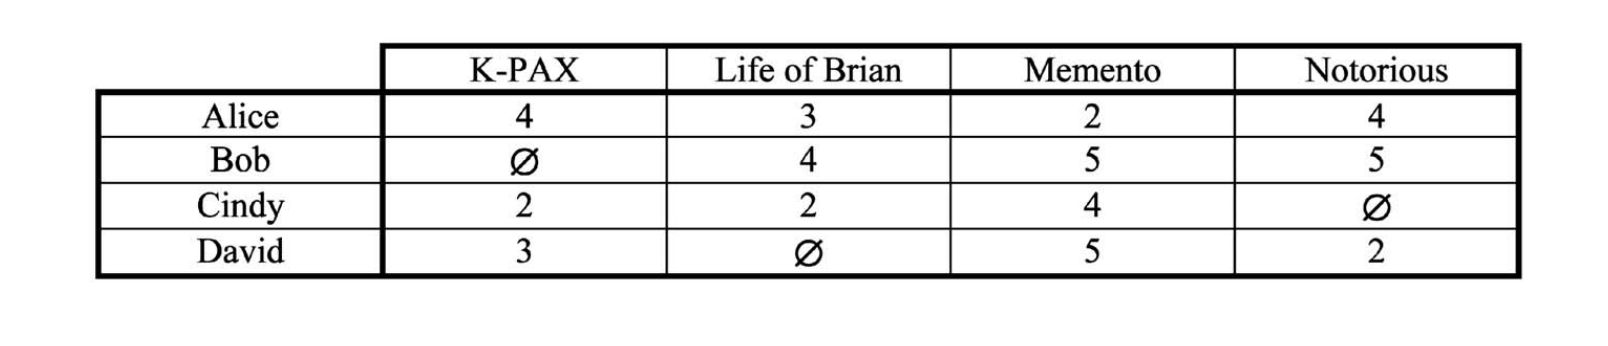
\includegraphics[scale=0.5]{chapters/figures/Rating Matrix.png}
    \caption{A snapshot of the rating matrix in a Movie Recommender System.  \\
    Source In: \textcite[735]{Adomavicius2005}}
    \label{fig:rating_matrix}
\end{figure}

\\

\emph{Hybrid Recommender System} are nothing but the combination of \emph{Content Based} and \emph{Collaborative Based} Recommender System which try to overcome their limitations \autocite[2]{Claypool1999CombiningCA}.\textcite[740]{Adomavicius2005} in their research work summarized the possible combinations in which \emph{Collaborative} and \emph{Content} based methods can be used to leverage their advantages. \textcite[5]{Claypool1999CombiningCA} in their work implemented a \emph{Hybrid Recommender System} for Online Newspaper recommendations and demonstrated that the \emph{Hybrid Recommender System} performed well in comparison to other methods. \\ \par

Types of Ratings
To date several researchers have investigated the area of Recommender System. Various study have stressed on the importance of the user-item preference and its influence on the recommendations. The most common way to capture such preference is via ratings, like/dislike  where users express their opinion. This valuable feedback data not only empowers service providers to evaluate their products / offerings from users viewpoint but also allows them to predict the interest or buying behaviour of \emph{users}. Moreover for users, the rating associated with an item provides helpful information which encourages them to investigate more about the \emph{item}. Literature on Recommender System suggests that the rating data can be classified into two broad categories namely: Explicit Feedback and Implicit Feedback\autocite[796]{Lak2014}.

\begin{figure}
    \centering
    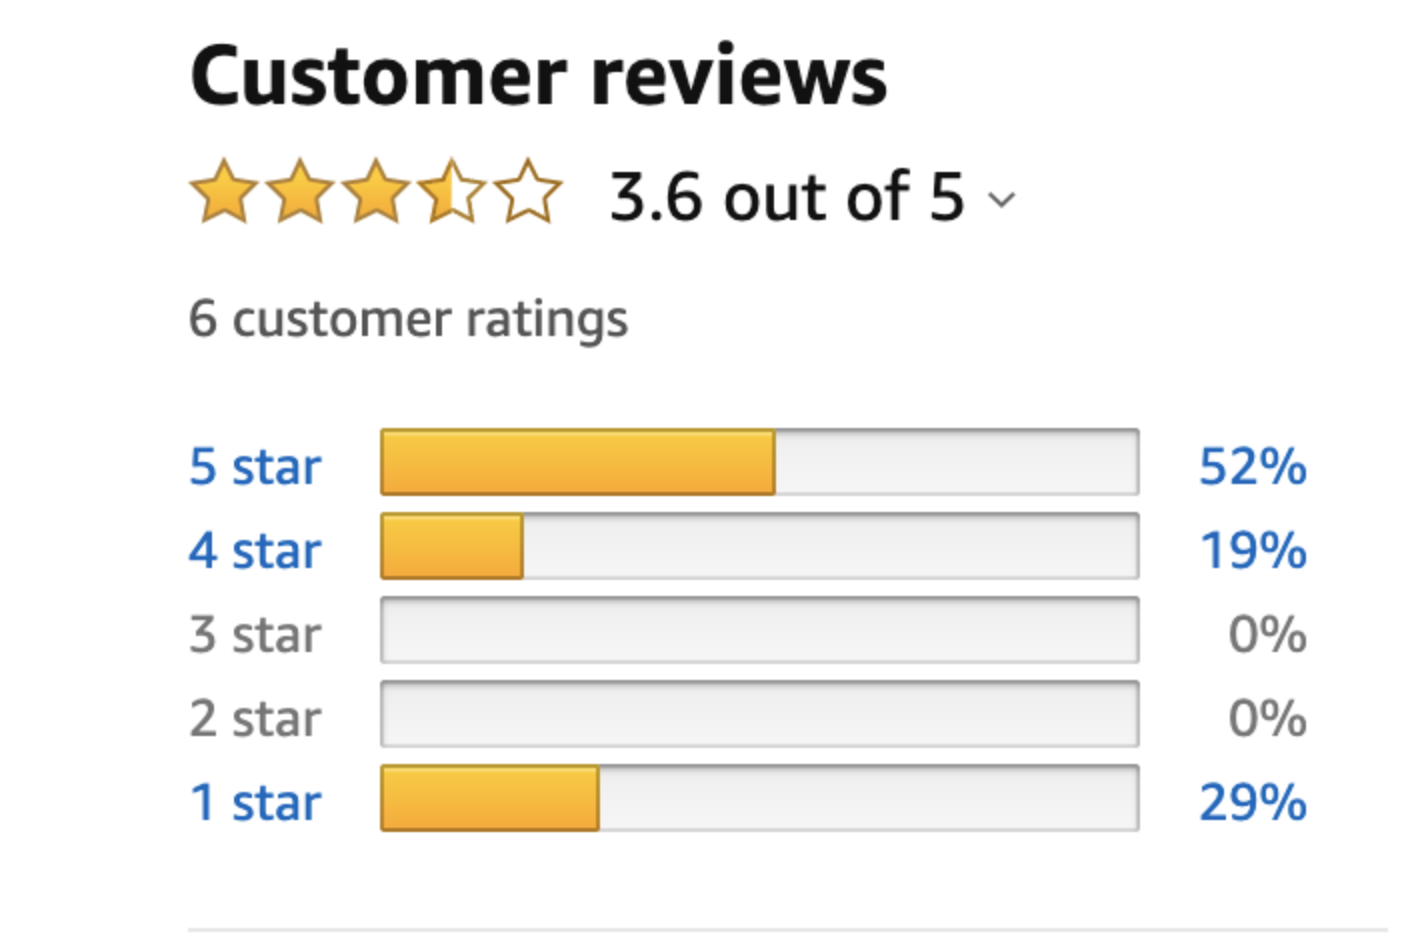
\includegraphics[scale=0.4]{chapters/figures/rating.png}
    \caption{An illustration of 5-star rating scale used by Amazon.\\
    Source: In www.Amazon.de}
    \label{fig:rating}
\end{figure}

\begin{itemize}
    \item Explicit Feedback refers to the opinion expressed by the \emph{users} which reflects a specific level of like or dislike towards the \emph{item}. Generally the ratings are designed on the basis of fixed set of ordered numbers which are used to measure the like or dislike\autocite[11]{Mertens1997}. For example a 5 star rating scale as illustrated in Fig\ref{fig:rating} 
    
    \item Implicit Feedback refers to data where the interest of \emph{users} is inferred from user activities such as browsing history, purchase history, or page-navigation patterns. Implicit Feedback describe the activities of the \emph{users} on the basis of the frequency of certain action such as number of times a particular product was bought\autocite[2]{Hu2008}. Unlike Explicit Feedback where the rating data reflects the \emph{users} preference, Implicit Feedback reflects \emph{users} confidence \autocite[2]{Hu2008}. For example, a user listening to a specific song probably indicates a strong affinity towards the artist, genre etc.
\end{itemize} 
\\
Although most of the research related to Recommender System is done using Explicit Feedback, there is a strong interest in using Implicit Feedback for recommendations. It is due to the fact that most of the times the detailed Explicit Feedback data is not available. Moreover the reliability of ratings obtained from \emph{users} is questioned as the \emph{users} may not be willing to provide genuine feedback unless there is strong motivation or reward associated with it \autocite[33]{Claypool1999CombiningCA}. In case of Implicit Feedback data there are challenges in utilizing it as compared to Explicit Feedback data, Implicit Feedback data does not express level of preference \autocite[2]{Hu2008}. Many researchers have proposed different algorithms which can handle Implicit Feedback data and have proved to be more useful in predicting the behavior of \emph{users} \autocite[2]{Koren2015}. \\


\section{Context Aware Recommender Systems}
In general it can be said that the main task of Recommender System is to predict the user preference for an item which he/she has never seen. Traditional Recommender System accomplish this by analyzing the user-item preferences which can be either obtained from users ratings or can be inferred from user activities. Based on this construct \textcite[8]{Adomavicius2011} defined the process of predicting the rating as follows \\
 \begin{center}
                \emph{R : User x Item \rightarrow Rating} \\
                \\
 \end{center}
     
Where \emph{User, 
Item} represent the set of users and items respectively and \emph{Rating} represents the predicted ratings denoted by non negative numbers bounded by a specific range. However, the ratings generated are only on the basis of the past user-item interaction data. Any other additional information is not considered in the recommendation process. This structure of traditional Recommender System makes it difficult to deliver the personalized content for e.g. recommending product based on the geographical location, time etc. Thus in order to make the recommendations more personalized and accurate to each user, additional information represented in the form of context can increase the prediction accuracy of the recommendation process \autocite[2]{Adomavicius2011}. A systematic study conducted by \textcite[1547]{Palmisano2008} proved that the use and importance of contextual information in modelling the \emph{users} behavior leading to high quality and accurate results. \\

The term \emph{context} is widely used across different domains counting Computer Science, Psychology, Linguistics, Business and Marketing. Therefore there are many definitions of \emph{context}. In general \emph{context} can be defined as conditions under which a user makes a certain decision. These conditions can be time, location etc. \textcite[3]{Chen2000} in their work formally defined \emph{context} as: 
\emph{"Context is the set of environment states and settings that either determines an application's behavior or in which an application event occurs and is interesting to the user."}  \\ \par

Given the extensively researched methods for conventional Recommender Systems and advantages of using contextual information, many researchers have actively investigated and proposed different methods to incorporate contextual information.\textcite[36]{Adomavicius2005} in their work presented a Multi Dimensional model approach capable of modelling different contextual information represented by dimensions. Recommender Systems which use contextual information along with ratings preferences are termed as \emph{Context-Aware Recommender System (CARS)}. \textcite[8]{Adomavicius2011} in his work formulated the rating prediction function for CARS as:
\\
\begin{center}
\emph{R: User x Items x Context \rightarrow  Ratings} \\    
\\
\end{center}
Where \emph{ Users, Items and Context} represent the set of users, items and contextual information respectively and \emph{Rating} represents the predicted ratings denoted by non negative numbers bounded by a specific range. \textcite[17]{Adomavicius2011} proposed that the contextual information can be included in the recommendation process in three different ways as shown in Fig  \ref{fig:cars_types}. The components being the \emph{user, item, context}, represented by U,I,C respectively and R represents the ratings generated.

\begin{figure}
    \centering
    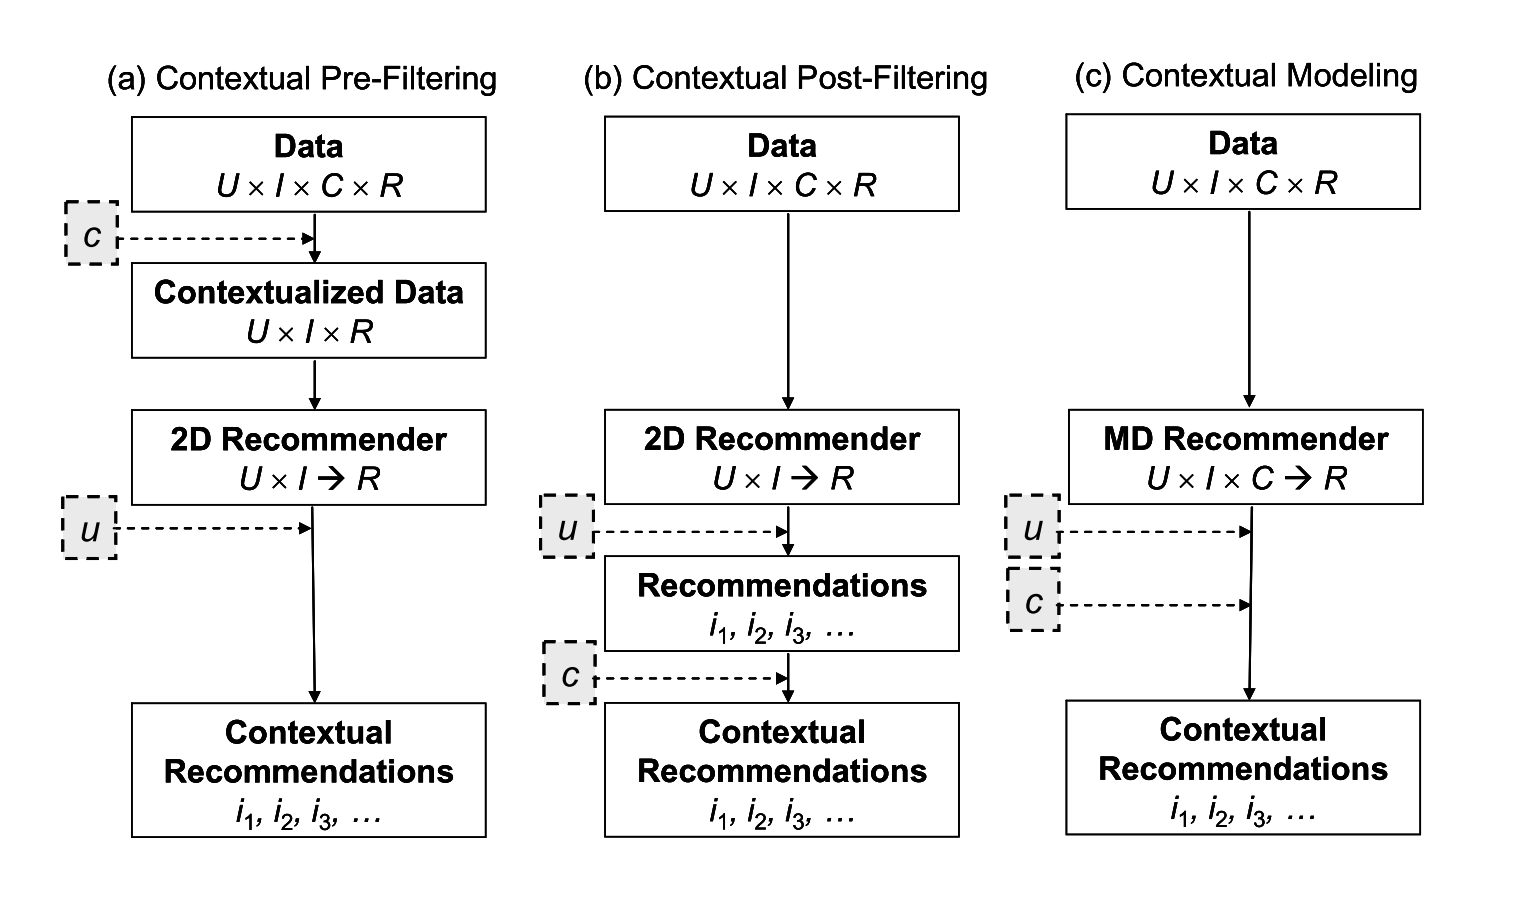
\includegraphics[scale=0.6]{chapters/figures/cars_types.png}
    \caption{Methods for including context in recommender systems.\\
    Source: In \textcite[17]{Adomavicius2011}}
    \label{fig:cars_types}
\end{figure}

\emph{Contextual Pre-Filtering}. This method first identifies the subset of user-item preference data based on the contextual information. The selected subset referred as \emph{Contextualized Data} is then feed to a traditional Recommender System to generate appropriate contextual recommendations. \\

\emph{Contextual Post-Filtering}. As the name suggests the contextual information is used as a filter after the the traditional Recommender System generates recommendations.  \\

\emph{Contextual Modeling}. This method combines the contextual information with the user-item preference data to generate contextual recommendations. Unlike Contextual Pre and Post Filtering methods, Contextual Modeling methods use more advance algorithms capable of including the contextual information in the recommendation process. 


\section{Personalization and Hyper Personalization}
Mass marketing has been one of the most widely used marketing strategies in the past to reach out to a more significant segment of the population. Easily accessible channels such as newspapers, radio, television assisted in widespread adoption of mass marketing strategies. With time, the marketing strategy evolved from broader mass marketing to more personal, one-to-one marketing. \textcite[306]{Arora2008} referred to personal one-to-one marketing tactic as personalization. The gradual shift from mass marketing to personalization is mainly propelled because of the expected benefits of personalization like higher profits, consumer loyalty and customer retention. Considering the perceived benefits of personalization and the fierce competitive environment, many companies are adopting one-to-one marketing strategies over mass marketing ones \autocite[409]{Vesanen2007}. \\ \par


Awareness of personalization is not recent, having possibly first described in the literature in the late 1950s \autocite[4]{WendellRSmith1956}. The form of personalization at that time addressed the consumers with their first name. Slowly with time this form of personalization changed. It gained momentum because of multiple factors, namely increased market competition, development in Information Technology capabilities, and widespread use of Peer-to-Peer communication capabilities \autocite[540]{Kumar2007}. Among service companies, personalization strategies are more widely adopted. For example, companies such as Amazon, eBay, Google Advertisement and News already have an implementation of personalization strategies to attract more users. \\ \par

%\begin{figure}
%    \centering
%    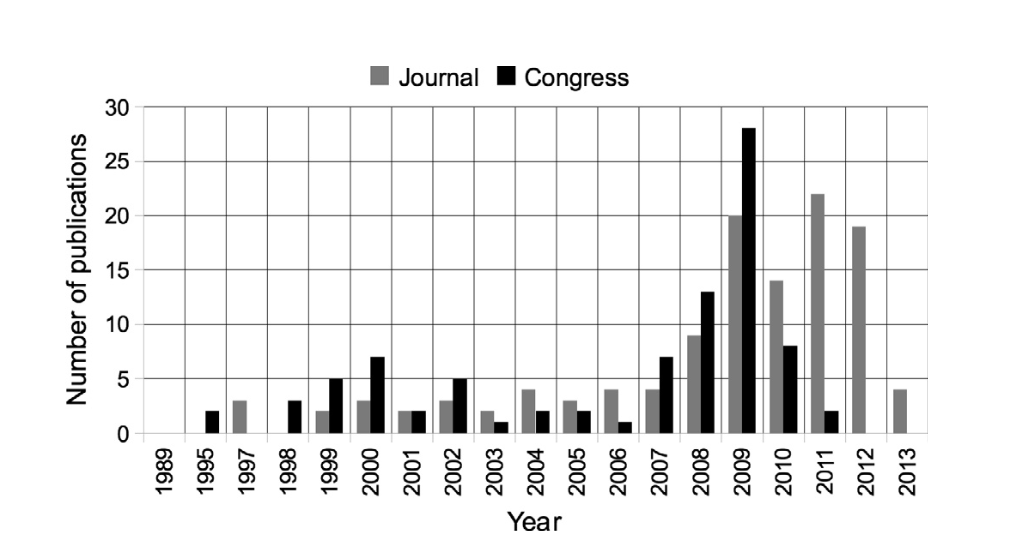
\includegraphics[scale=0.5]{chapters/figures/recommender_system_research_papers_Recommender systems survey J. Bobadilla ⇑, F. Ortega, A. Hernando, A. Gutiérrez.png}
%    \caption{Personalization process overview. \\
%    Source: In \autocite[10]{VesanenRaulas2007}}
%    \label{fig:Personalization_process}
%\end{figure}

Personalization concept is interdisciplinary involving the fields of Economics, Computer Science, Marketing, Operations Analysis \autocite[1344]{Murthi2003}. As a result, several researchers have extensively studied it in different contexts. The existing literature review on personalization is extensive and reveals multiple definitions used. \textcite[412]{Vesanen2007} conducted a systematic literature review and summarised the broad spectrum of definition found in the literature. It is also observed that literature, multiple terms such as one-to-one marketing, mass customization, segmentation, filtering, segmentation are used for defining personalization \autocite[2]{Montgomery2009}. Since many sectors have adopted personalization, the definition specific to e-commerce sector is considered concerning the theme of this study.\textcite[305]{Arora2008} defines personalization as tailoring the products or services offered by companies according to the needs of the individual consumer. It is often found that personalization and customization is used synonymous. Although these marketing strategies are related to one-to-one marketing strategies, there exits a subtle difference between them. \textcite[538]{Kumar2007} in his work elaborated the main difference between them. Customization is consumer initiated process, where as personalization is an automated process that intends to surprise the consumer. Most commonly found example of customization is in the automobile industry where consumers can effectively choose from the list of options and customize their vehicle. On the other hand personalization intends to identify the preferences of the user based on analyzing the consumer data such as his/her purchase history, ratings, reviews. To achieve this statistical methods are used to model the user preferences \autocite[310]{Arora2008}. An exemplary example of personalization can be found in e-commerce websites such as Amazon, where appropriate products are suggested to the user by analyzing the user information such as purchase history. \\ \par


\begin{figure}
    \centering
    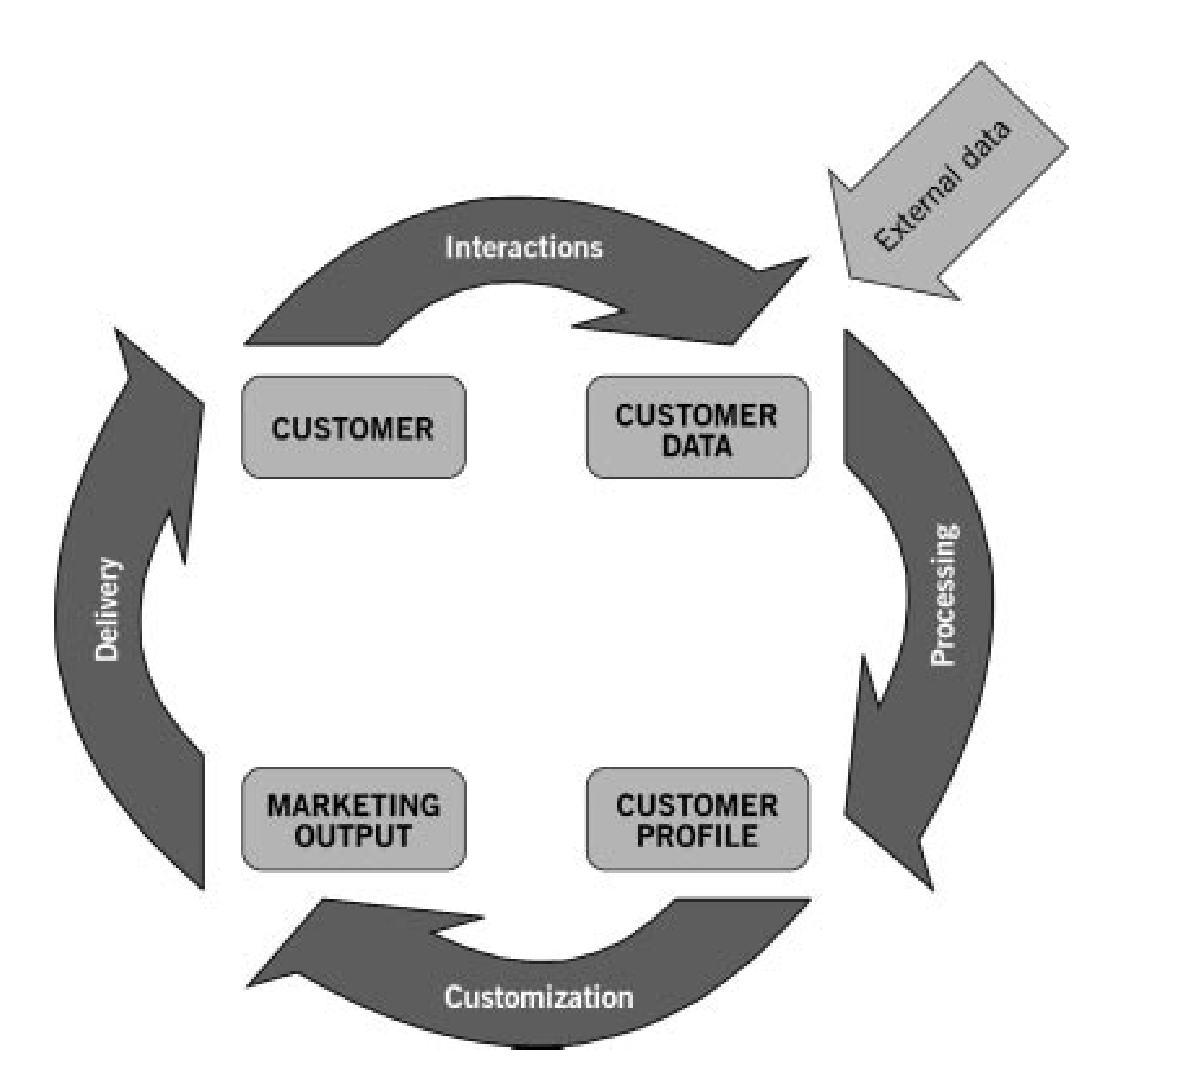
\includegraphics[scale=0.5]{chapters/figures/Personalization_process.png}
    \caption{Personalization process overview. \\
    Source: In \autocite[10]{VesanenRaulas2007}}
    \label{fig:Personalization_process}
\end{figure}


Implementing personalized marketing strategy has been a pain-point for marketers. One of the possible reason being that personalization can be interpreted in different ways due to its inter-disciplinary nature. Furthermore it is difficult for advertisers to enforce personalization in the absence of a standard framework. Numerous researchers have suggested various strategies for personalization process to respond to these challenges. \textcite[18]{Wind2001} identified the primary drivers of personalization namely: customer data, information technology, operational capabilities. In addition to this, \textcite[7]{VesanenRaulas2007} summed up the common element (as shown in Table \ref{tab:template}) required to implement personalization marketing where each object defined represents the necessary element and each operation defines the action performed on that element. In order to complete the personalization process, the elements communicate iterative with each other and supported by external data indicating various factors, as shown in the Fig \ref{fig:Personalization_process}.  \\ \par

\begin{table}[t]
\centering
\begin{tabular}{|l|c|}
\hline
Objects & Operations\\
\hline\hline
Customer & Interactions\\
\hline
Customer Data  &  Processing(analysis, data mining, targeting)\\
\hline
Customer Profile  & Customization\\
\hline
Marketing output  & Delivery\\
\hline
\end{tabular}
\centering
\caption{
Variables used in the Personalization process.\\
Source: In \autocite[8]{VesanenRaulas2007}}
\label{tab:template}
\end{table}

Throughout the entire process of personalization, the Information Technology dimension definitely plays an important role. It is required right from capturing the interactions of customers along with customer data, t processing them, analyzing them and finally deliver the insights. This process is possible only due to the recent advancements in processing huge amount of consumer data. Peer to Peer networking tools made it possible for peers to exchange knowledge / information in form of text, audio,video easy and seamless. Thus the widespread used of such Peer to Peer networking tools in applications such as e-commerce websites, mobile applications have supported to gather consumer data efficiently. New technological paradigm such as Big Data, Machine Learning and Artificial Intelligence have proved their capabilities in processing and analyzing massive database. An application of such technology is found in Recommender Systems which utilize statistical methods and Machine Learning algorithms to model user profiles which are used in personalization process\autocite[4]{Adomavicius2011}. Recommender Systems can effectively analyze the consumer data and generate personalized set recommendations of items/services for each user. Considering the e-commerce or online service industry, the personalization process is not only limited to the recommendation of certain products but also include a personalized price of goods, promoting less known but quality products and up-selling. \autocite[203]{zhang2009effectiveness} \\ \par 

A considerable amount of literature published on personalization has emphasized on the  effectiveness of personalization leading to increased revenues, customer retention and higher satisfaction. A case-study research reveal similar findings where companies employing personalization achieve higher customer satisfaction \autocite[33]{Jackson2007}. Personalization technology provide consistent, timely and relevant information when required by the customer. Such personalized experience not only creates a value for the customer but also satisfies the needs of customer. From the point of view of the businesses operating in the field of e-commerce, the reduction in the operational costs of technology associated with the introduction of personalization has led to a widespread acceptance of the strategy. Consequently, personalization in the form of product recommendations is widely adopted among the modern applications such as e-commerce, music streaming websites. \\ 
\par


As discussed earlier the improved capabilities in aggregating data from different sources and processing and analyzing them has allowed researchers to explore personalization from different perspectives. One such perspective is to include the contextual data in modelling of the user preferences. Contextual data refers to the information such as time, mood of the person, season etc. under which a activity is performed by the user. By considering contextual factors in the personalization process, a product offering or marketing strategy can be tailored as per the needs of the customer. Generating real-time and contextualized recommendations at individual level is nothing but Hyper-personalization \autocite[5]{CapgeminiconsultingESSECBusinessSchool2016}. Although there is no specific definition for the term Hyper-Personalization, the above mentioned definition suits well in the context of e-commerce domain. The argument for including contextual information is drawn from behavioral science which states that the consumers decision making process is influenced by the underlying environmental conditions in which a particular action is performed or observed \autocite[174]{foxall2001foundations}. A study conducted by \textcite[332]{Jain2018} found that Hyper-personalized web-pages have strong relationship with an intention to purchase.
Thus, predicting the actions of the users or adjusting the marketing strategy based on the conditions is the main gist of the contextualized personalization process. \\ 
\par
Hyper-personalization is still in its early stages of it conception and it is being continuously developed and tested. It is often used as a general term covering different areas. Literature search on the topic of Hyper-personalization results in few relevant research papers. This can also be considered as indicator for the initial stages of this topic. Having said that, the concept of Hyper-Personalization can be closely related to the use of different technologies such as Radio Frequency Identification (RFID),Internet of Things devices, Machine learning and Data Mining, Virtual Reality ,Locations based systems, etc to enhance the consumer experience as mentioned in the research work of \textcite[2]{Faulds2018}.  The rising interest in the topic of Hyper-personalization is fuelled by the advancements in the field of Machine learning and Data Mining as well as the need to need to predict or analyze the consumer behavior to delivery an exemplary customer experience\autocite[]{CapgeminiconsultingESSECBusinessSchool2016}. A survey conducted by BCG found that \% of the companies think that it is hyper-personalization implementation will help them boost the revenue and attract new customer. Companies that wish to take advantage of this technology, first need to better understand their customers, their needs and demands. Consumers demand an experience which is tailor made for them considering their interest areas \autocite[6]{CapgeminiconsultingESSECBusinessSchool2016}. Considering these circumstances, the personalization strategies developed in the past considered factors like demographics, age-group etc. which generalize the services or product offering often to a section of the consumers base will not be effective anymore \autocite[6]{CapgeminiconsultingESSECBusinessSchool2016}. As a consequence companies must redesign marketing strategies that focus at an individual consumer level with keeping in mind the needs of the consumers. Hyper-personalization approach supports this idea by using sophisticated mix of technology such as Machine Learning and Data Mining. The following sub-chapter describes more on the use of technology in the inception of Hyper-personalization.


\section{Machine Learning approach on Hyper-Personalization}
The capability of Machine Learning and Data Mining methods in analyzing the patterns in large quantity of data has made it ideal for developing large and scalable applications \autocite[2]{Sodhi}. With the help of such applications companies can extract insights about their customers and product and can quickly adapt their marketing strategies. For e.g. Amazon personalizes the home page of their website for each of its user which includes seasonal offers and discounts on products as seen in Fig \ref{fig:amazon_home_page}. A report by \textcite[20]{DHL2019} on Hyper-Personalization suggests that the first step to move towards Hyper-Personalization is to know the customers base and gather data at different touch points in the customer journey. By collecting such detailed information from different interaction channels, previous transactions and explicit ratings and review can help in predicting the consumer behaviour, understand their interest areas and identify new opportunities \autocite[20]{DHL2019}. Furthermore, from the perspective of companies such insights help in better planning of the inventory activities and minimize the cost associated with it. \\ 
\par
%To implement the Hyper-personalized system, technologies such as Big Data and Machine %Learning can be leveraged as to collect data of its customers. \autocite[2]{Sodhi}.
 Big Data technologies aggregate huge amounts of data received from different source whereas Machine Learning helps in identifying insights from the data. Additionally, \textcite[2]{Sodhi} also suggested that when these technology driven process are implemented in an agile way, it not only gives the companies the flexibility but also the provides an opportunity to experiment with different ideas and strategies. \\
\par
Creating a Hyper-personalized experience for the consumers is largely dependent on the amount and quality of the user-data that is available. A high quality, detailed and diverse data of users is always desirable as it helps in modelling different scenarios and covers wide spectrum of customer behavior \autocite[8]{CapgeminiconsultingESSECBusinessSchool2016}. Additionally, the widespread use of mobile devices, Internet of Thing devices (IoT) enables in capturing behavioral data which can be used to develop high quality applications such as Recommender Systems \autocite[8]{CapgeminiconsultingESSECBusinessSchool2016}. Such systems rely on Machine Learning algorithms which can integrate not only the purchase data but also other contextual information to generate accurate recommendations \autocite[67]{Adomavicius2011}. The data-driven applications is not only limited to Recommender Systems. \autocite[3]{Sodhi} in his work suggested that combining the predictive power of the Machine Learning algorithms and high quality data of the customers, applications such as Data Management Platforms which help in automated targeted advertising, Marketing Automation Platform which enables real-time behaviour analysis can be derived. Apart from that, to truly make the customer journey Hyper-personalized, different applications such chat-bot, costumer sentiment analysis can be deployed.


Such high quality data can be used to derive applications such as Web Personalization and Recommender Systems, Data Management Platforms, Marketing Automation Platforms \autocite[3]{Sodhi}. Recommender Systems 
Such applications are typically powered by Machine Learning algorithms. 

A study conducted by \textcite{Bradley2015} weighted on the premise that  ".. insight is currency and context is king"
- Machine Learning transforming Marketing industry
- what are the types of machine learning model that can be used to implement hyper-personalization

 
\begin{figure}
    \centering
    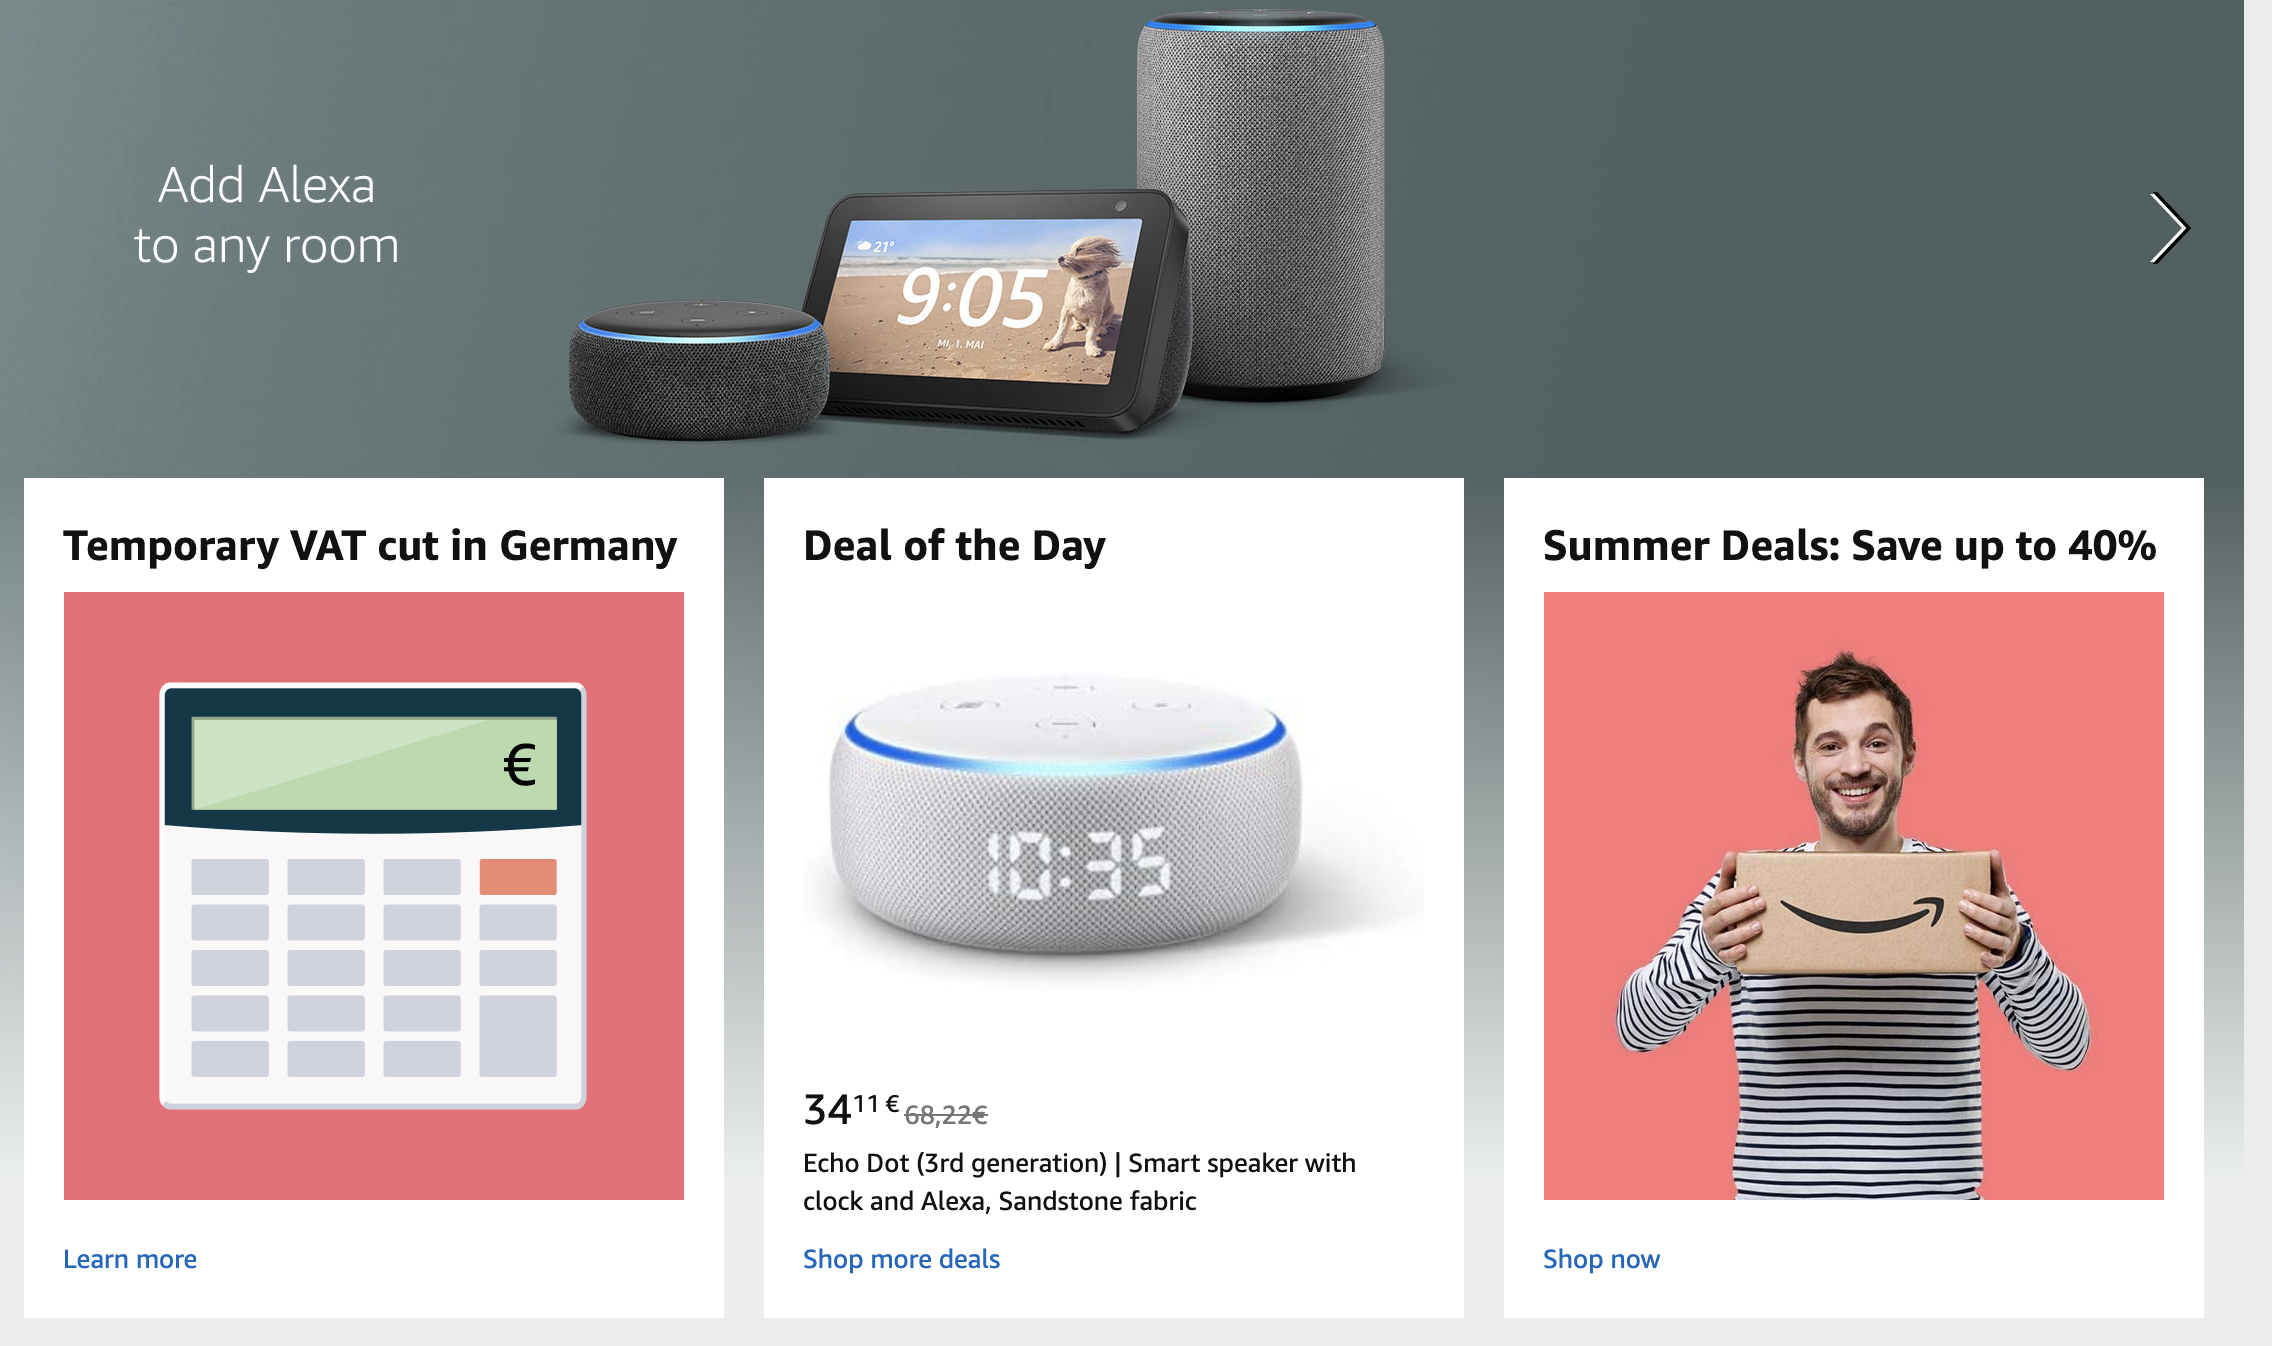
\includegraphics[scale=0.3]{chapters/figures/amazon_homepage.png}
    \caption{Personalization of home-page. \\
    Source: In www.amazon.de}
    \label{fig:amazon_home_page}
\end{figure}
